\chapter{Análise Univariada}

\section{Introdução}
A \textbf{análise univariada} é o estudo de uma variável por vez, com o objetivo de compreender sua distribuição, valores típicos e dispersão.  
Ela é a base da \textbf{estatística descritiva}, responsável por organizar, resumir e apresentar dados de forma clara.  

De modo geral, a \textbf{estatística} se divide em duas grandes áreas:  
\begin{itemize}[leftmargin=*]
  \item \textbf{Estatística descritiva}: coleta, organização, resumo e apresentação de dados;  
  \item \textbf{Estatística inferencial}: técnicas que permitem generalizar conclusões de uma amostra para a população (ex.: testes de hipóteses, intervalos de confiança).  
\end{itemize}

Na AED, a estatística descritiva é essencial para “deixar os dados falarem” antes da aplicação de modelos mais sofisticados.

\section{Conjuntos e Tipos de Variáveis}
Antes de calcular medidas, é preciso reconhecer o tipo de variável:  
\begin{itemize}[leftmargin=*]
  \item \textbf{Qualitativas}: categóricas, não numéricas (ex.: sexo, estado civil, cidade);  
  \item \textbf{Quantitativas discretas}: assumem valores inteiros contáveis (ex.: número de filhos, horas de estudo);  
  \item \textbf{Quantitativas contínuas}: assumem valores em intervalos reais (ex.: altura, renda, temperatura).  
\end{itemize}

Exemplo de conjunto de dados (adaptado da prova):  

\begin{center}
\begin{tabular}{@{}lccccc@{}}\toprule
Aluno & A & B & C & D & E \\\midrule
Horas de Estudo & 8 & 4 & 2 & 1 & 10 \\
Nota Final      & 8 & 6 & 2 & 1 & 10 \\\bottomrule
\end{tabular}
\end{center}

\section{Medidas de Posição}

\subsection*{Média}
\begin{FormulaBox}
Média aritmética: $\quad \bar{x} = \frac{1}{n}\sum_{i=1}^{n}x_i$
\end{FormulaBox}

Exemplo (Notas):  
\[
\bar{y} = \frac{8+6+2+1+10}{5} = \frac{27}{5} = 5{,}4
\]

\subsection*{Mediana}
\begin{FormulaBox}
Mediana ($\tilde{x}$): valor central dos dados ordenados.  
Se $n$ é ímpar, $\tilde{x}$ é o valor central; se $n$ é par, é a média dos dois centrais.
\end{FormulaBox}

Exemplo (Horas): $\{1,2,4,8,10\}$ → $\tilde{x}=4$.

\subsection*{Moda}
\begin{FormulaBox}
Moda: valor que mais se repete no conjunto.  
Pode não existir (sem repetições) ou haver mais de uma moda (bimodal, multimodal).
\end{FormulaBox}

Exemplo: $\{2,2,4,5,6\}$ → moda = 2.

\paragraph{Média vs Mediana}
A média é sensível a valores extremos, enquanto a mediana é robusta a outliers.  OU seja, se a diferença entre média e mediana for grande, é um alto indício de existir outliers na base.
\begin{itemize}
  \item Dados: $\{10,12,14,15,500\}$  
  \item Média = 110,2 (influenciada pelo 500)  
  \item Mediana = 14 (representa melhor o centro dos dados)  
\end{itemize}

\section{Medidas de Dispersão}

\subsection*{Variância}
\begin{FormulaBox}
Variância amostral: $\quad s^2 = \frac{1}{n-1}\sum_{i=1}^{n}(x_i - \bar{x})^2$
\end{FormulaBox}

\subsection*{Desvio Padrão}
\begin{FormulaBox}
Desvio-padrão: $\quad s = \sqrt{s^2}$
\end{FormulaBox}

Exemplo (Notas):  
$s_y^2 = 14{,}8$; \quad $s_y \approx 3{,}85$

\section{Boxplot e Identificação de Outliers}

O \textbf{boxplot} é um gráfico que resume a distribuição de uma variável numérica utilizando \textbf{quartis} e limites de dispersão.  
Ele é muito útil para identificar a mediana, a variabilidade e a presença de \textbf{outliers}.

\begin{figure}[H]
\centering
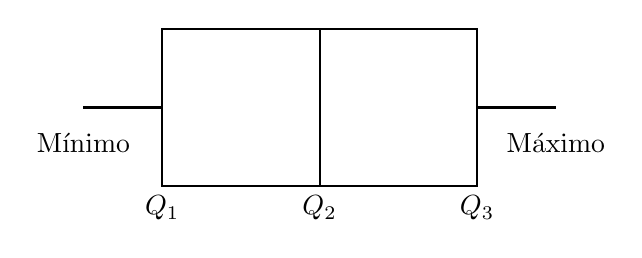
\begin{tikzpicture}
  % Caixa
  \draw[thick] (0,0) rectangle (4,2); % Q1 até Q3
  % Mediana
  \draw[thick] (2,0) -- (2,2);
  % Whiskers
  \draw[thick] (0,1) -- (-1,1);
  \draw[thick] (4,1) -- (5,1);
  \draw[-] (-1,1) -- (0,1);
  \draw[-] (4,1) -- (5,1);
  % Legendas
  \node[below] at (0,0) {$Q_1$};
  \node[below] at (2,0) {$Q_2$};
  \node[below] at (4,0) {$Q_3$};
  \node[below] at (-1,0.8) {Mínimo};
  \node[below] at (5,0.8) {Máximo};
\end{tikzpicture}
\caption{Representação esquemática de um boxplot.}
\end{figure}

\subsection*{Passo a Passo para Construir um Boxplot}
\begin{enumerate}[leftmargin=*]
  \item \textbf{Calcular $Q_1$, $Q_2$ e $Q_3$}:  
  - $Q_1$ (1º quartil) é o valor abaixo do qual estão 25\% dos dados.  
  - $Q_2$ (mediana) é o valor central (50\%).  
  - $Q_3$ (3º quartil) é o valor abaixo do qual estão 75\% dos dados.  
  *(Os detalhes de cálculo dos percentis estarão no Apêndice do capítulo).*
  
  \item \textbf{Encontrar os valores mínimo e máximo gerais da amostra}.  

  \item \textbf{Calcular o intervalo interquartil (IQR)}:
  \begin{FormulaBox}
  $IQR = Q_3 - Q_1$
  \end{FormulaBox}

  \item \textbf{Determinar limites inferior e superior usando o IQR}:
  \begin{FormulaBox}
  $\text{Mín\_IQR} = Q_1 - 1,5 \times IQR$ \\[4pt]
  $\text{Máx\_IQR} = Q_3 + 1,5 \times IQR$
  \end{FormulaBox}

  \item \textbf{Calcular os whiskers}:  
  - O \textbf{mínimo do boxplot} será o maior valor entre o mínimo geral e $\text{Mín\_IQR}$.  
  - O \textbf{máximo do boxplot} será o menor valor entre o máximo geral e $\text{Máx\_IQR}$.  
  Valores além desses limites são representados como \textbf{outliers}.
\end{enumerate}

Esse processo garante que a caixa represente a maior parte dos dados (50\% entre $Q_1$ e $Q_3$), mas que valores muito extremos não distorçam a visualização.  
Assim, o boxplot é uma ferramenta robusta contra outliers, diferentemente da média e do desvio-padrão.


\section{Problemas Resolvidos — Questões 2 e 3}

\subsection*{Questão 2 — Cálculo de média, mediana, variância e desvio-padrão}

\begin{SolvedBox}
\textbf{Contexto.} Uma equipe coletou \emph{Horas de estudo} ($x$) e \emph{Notas finais} ($y$) de 5 participantes. Queremos: (i) calcular as \textbf{médias} de $x$ e $y$; (ii) as \textbf{medianas}; (iii) a \textbf{variância amostral} e o \textbf{desvio-padrão} de cada variável.

\textbf{Passo 1 — Tabela de dados}\\[-6pt]
\begin{center}
\begin{tabular}{@{}lccccc@{}}\toprule
Registro & R1 & R2 & R3 & R4 & R5 \\\midrule
Horas ($x$) & 8 & 4 & 2 & 1 & 10 \\
Notas ($y$) & 8 & 6 & 2 & 1 & 10 \\\bottomrule
\end{tabular}
\end{center}

\textbf{Passo 2 — Cálculo das médias}

\begin{FormulaBox}
Média: $\quad \bar{x} = \dfrac{\sum x_i}{n}, \qquad \bar{y} = \dfrac{\sum y_i}{n}$
\end{FormulaBox}

\[
\bar{x} = \frac{8+4+2+1+10}{5} = \frac{25}{5} = 5,
\qquad
\bar{y} = \frac{8+6+2+1+10}{5} = \frac{27}{5} = 5{,}4
\]

\textbf{Passo 3 — Medianas (dados ordenados)}\\
Horas ordenadas: $\{1,2,4,8,10\} \Rightarrow \tilde{x}=4$. \quad
Notas ordenadas: $\{1,2,6,8,10\} \Rightarrow \tilde{y}=6$.

\textbf{Passo 4 — Tabela para variância e desvio-padrão (Horas)}

\begin{center}
\begin{tabular}{@{}c|c|c@{}}\toprule
$\,x_i\,$ & $x_i - \bar{x}$ & $(x_i - \bar{x})^2$ \\\midrule
8  & 3   & 9 \\
4  & -1  & 1 \\
2  & -3  & 9 \\
1  & -4  & 16 \\
10 & 5   & 25 \\\midrule
\textbf{Soma} & --- & \textbf{60} \\\bottomrule
\end{tabular}
\end{center}

\begin{FormulaBox}
Variância amostral: $\quad s_x^2 = \dfrac{\sum (x_i - \bar{x})^2}{n-1}$ \qquad
Desvio-padrão: $\quad s_x = \sqrt{s_x^2}$
\end{FormulaBox}

\[
s_x^2 = \frac{60}{5-1} = \frac{60}{4} = 15,
\qquad
s_x = \sqrt{15} \approx 3{,}873
\]
\end{SolvedBox}

\begin{SolvedBox}
\textbf{Passo 5 — Tabela para variância e desvio-padrão (Notas)}



\begin{center}
\begin{tabular}{@{}c|c|c@{}}\toprule
$\,y_i\,$ & $y_i - \bar{y}$ & $(y_i - \bar{y})^2$ \\\midrule
8  & 2{,}6  & 6{,}76 \\
6  & 0{,}6  & 0{,}36 \\
2  & -3{,}4 & 11{,}56 \\
1  & -4{,}4 & 19{,}36 \\
10 & 4{,}6  & 21{,}16 \\\midrule
\textbf{Soma} & --- & \textbf{59{,}2} \\\bottomrule
\end{tabular}
\end{center}



\begin{FormulaBox}
Variância amostral: $\quad s_y^2 = \dfrac{\sum (y_i - \bar{y})^2}{n-1}$ \qquad
Desvio-padrão: $\quad s_y = \sqrt{s_y^2}$
\end{FormulaBox}

\[
s_y^2 = \frac{59{,}2}{4} = 14{,}8,
\qquad
s_y = \sqrt{14{,}8} \approx 3{,}85
\]

\textbf{Resumo (como eu apresentaria na resposta):}
\begin{itemize}[leftmargin=*]
  \item $\bar{x}=5$, $\tilde{x}=4$, $s_x^2=15$, $s_x\approx 3{,}873$;
  \item $\bar{y}=5{,}4$, $\tilde{y}=6$, $s_y^2=14{,}8$, $s_y\approx 3{,}85$.
\end{itemize}
\end{SolvedBox}

% ------------------------------------------------------------

\subsection*{Questão 3 — Construção do boxplot das notas}

\begin{SolvedBox}
\textbf{Contexto.} Usando as mesmas \emph{Notas} do conjunto acima, deseja-se construir o \textbf{boxplot}. Os valores de $Q_1$, $Q_2$ e $Q_3$ são informados pelo professor.

\textbf{Passo 1 — Dados ordenados e quartis dados}\\
Notas ordenadas: $\{1,2,6,8,10\}$ \quad (fornecido) $Q_1=2,\; Q_2=6,\; Q_3=8$.

\textbf{Passo 2 — Intervalo interquartil (IQR)}

\begin{FormulaBox}
$IQR = Q_3 - Q_1$
\end{FormulaBox}

\[
IQR = 8 - 2 = 6
\]

\textbf{Passo 3 — Limites por IQR (para outliers)}

\begin{FormulaBox}
\text{Mín\_IQR} = Q_1 - 1{,}5 \times IQR \qquad
\text{Máx\_IQR} = Q_3 + 1{,}5 \times IQR
\end{FormulaBox}

\[
\text{Mín\_IQR} = 2 - 1{,}5\times 6 = -7
\qquad
\text{Máx\_IQR} = 8 + 1{,}5\times 6 = 17
\]

\textbf{Passo 4 — Whiskers (mín e máx do boxplot)}\\
Mínimo geral = $1$, Máximo geral = $10$.\\
\emph{Regra:} 
\begin{itemize}[leftmargin=*]
  \item \textbf{Mínimo do boxplot} = $\max(\text{mínimo geral}, \text{Mín\_IQR}) = \max(1,-7)=1$;
  \item \textbf{Máximo do boxplot} = $\min(\text{máximo geral}, \text{Máx\_IQR}) = \min(10,17)=10$.
\end{itemize}
Como $1$ e $10$ estão \emph{dentro} de $[-7,17]$, \textbf{não há outliers}.

\textbf{Passo 5 — Desenho esquemático (valores indicados)}\\[-4pt]
\begin{figure}[H]
\centering
\begin{tikzpicture}[x=0.6cm,y=0.6cm]
  % Eixo base (0 a 11 para visual)
  \draw[gray!60] (-1,0) -- (11,0);
  \foreach \x in {0,...,10} \draw[gray!60] (\x,0.1) -- (\x,-0.1) node[below] {\scriptsize \x};

  % Caixa Q1 a Q3
  \filldraw[fill=pastelblue, draw=black] (2,1) rectangle (8,3); % Q1=2, Q3=8
  % Mediana
  \draw[very thick] (6,1) -- (6,3); % Q2=6
  % Whiskers
  \draw[thick] (1,2) -- (2,2); % min whisker
  \draw[thick] (8,2) -- (10,2); % max whisker
  % Pontos rotulados
  \node[below] at (2,1) {\scriptsize $Q_1=2$};
  \node[below] at (6,1) {\scriptsize $Q_2=6$};
  \node[below] at (8,1) {\scriptsize $Q_3=8$};
  \node[below] at (1,0) {\scriptsize min=1};
  \node[below] at (10,0) {\scriptsize max=10};
\end{tikzpicture}
\caption{Boxplot das notas com $Q_1=2$, $Q_2=6$, $Q_3=8$, whiskers em 1 e 10.}
\end{figure}

\textbf{Como eu escreveria a interpretação:} a metade central dos dados está entre $2$ e $8$ (IQR=6), a mediana é $6$, e não há outliers.
\end{SolvedBox}

\clearpage
\section*{Problemas Sugeridos — Praticando Análise Univariada}

\begin{enumerate}[leftmargin=*]

  \item Considere as idades $\{18, 20, 21, 23, 30\}$.  
  Calcule média, mediana e moda. Interprete se a média ou a mediana representa melhor o grupo.

  \item Para os salários mensais $\{2000, 2200, 2300, 2400, 15000\}$, calcule média, mediana, variância e desvio-padrão.  
  Verifique se há outlier com base no boxplot.

  \item Dada a série de notas $\{5, 7, 8, 9, 10\}$:  
  Calcule o intervalo interquartil (IQR) e os limites inferior e superior (Mín\_IQR e Máx\_IQR).

  \item Considere os tempos de atendimento em minutos $\{3, 4, 5, 6, 25\}$.  
  Construa o boxplot (informe $Q_1, Q_2, Q_3$) e interprete o impacto do valor 25.

  \item Uma pesquisa registrou a quantidade de livros lidos em um mês por 6 pessoas: $\{0, 1, 2, 2, 3, 10\}$.  
  Calcule média, mediana, variância e desvio-padrão. Interprete.

  \item Para os dados de temperatura $\{21, 22, 22, 23, 24, 25, 40\}$, calcule a média, o desvio-padrão e verifique se há outlier pelo método do IQR.

  \item Uma base contém os valores de vendas (em milhares de reais): $\{15, 16, 16, 17, 18, 100\}$.  
  Construa o boxplot e indique se 100 é ou não um outlier.

  \item Dada a sequência de alturas (cm) $\{150, 155, 160, 165, 170, 175, 180\}$, calcule média, mediana, variância e desvio-padrão.  
  Interprete a simetria dos dados.

  \item Um conjunto de dados registra a quantidade de horas de sono por noite: $\{5, 6, 7, 7, 8, 9, 10\}$.  
  Calcule a média e o desvio-padrão. Qual a interpretação prática de $s$ neste contexto?

  \item Considerando os valores de consumo de energia (kWh): $\{120, 125, 130, 135, 200\}$, construa o boxplot.  
  Explique como a presença do valor 200 altera a interpretação dos dados.

\end{enumerate}







\section*{Apêndice — Cálculo de Percentis e Quartis}
\begin{ProofBox}
\textbf{O que são percentis?}  
Percentis são medidas de posição que dividem um conjunto de dados ordenados em 100 partes iguais.  
- O percentil $p$ indica o valor abaixo do qual está $p\%$ das observações.  
Exemplo: o percentil 90 ($P_{90}$) é o valor abaixo do qual estão 90\% dos dados.  

\medskip
\textbf{Como calcular percentis (método clássico):}  
\[
\text{Posição}(p) = \frac{p}{100} \times (n+1)
\]
onde $n$ é o número de observações e $p$ é o percentil desejado.  

- Se a posição for um número inteiro, o percentil corresponde exatamente ao valor nessa posição dos dados ordenados.  
- Se a posição não for inteira, o valor é obtido por \textbf{interpolação linear} entre os dois valores mais próximos.  

\medskip
\textbf{Exemplo:}  
Para $n=10$ observações e $p=25$:  
\[
\text{Posição}(25) = \frac{25}{100}(10+1) = 2,75
\]  
Isso significa que $Q_1$ (percentil 25) está entre o 2º e o 3º valor da lista ordenada, a 75\% da distância entre eles.

\medskip
\textbf{Quartis como casos especiais de percentis:}  
- $Q_1 = P_{25}$: 25\% dos dados estão abaixo.  
- $Q_2 = P_{50}$: mediana (50\% dos dados abaixo e 50\% acima).  
- $Q_3 = P_{75}$: 75\% dos dados estão abaixo.  

\medskip
\textbf{Observação prática:}  
Na estatística aplicada e em softwares (R, Python, Excel, SQL), existem diferentes métodos para cálculo de percentis, que podem variar no uso de $n$ ou $n+1$ na fórmula.  
Na AED, o importante é manter a consistência no método escolhido.
\end{ProofBox}

